\chapter{Application: prédiction d'entrée manquante}
\graphicspath{{05-Application/}}
\minitoc

Une façon d'appliquer la mémoire associative de l'architecture de cartes est de prédire une modalité. Une architecture de cartes se comporte comme un système dynamique, réagissant aux entrées présentées.
Grâce à l'aspect réciproque des connexions, une activité peut être calculée dans une carte ne recevant pas d'entrée externe.
Nous montrerons dans ce chapitre que CxSOM permet de prédire une entrée manquante sur une des cartes, de façon dynamique, sans utiliser d'algorithme prédictif supplémentaire. On utilise le même algorithme que celui de test, mais en n'utilisant simplement pas l'entrée externe d'une des carte pourle calcul du BMU. Le poids du BMU de cette carte devient alors une prédiction de l'entrée manquante, générée par les connexions entre cartes.

\section{Prédiction d'entrées géométriques}

\subsection{Méthodes}

Nous expérimentons d'abord la prédiction sur les données géométriques $X,Y,Z$ utilisées précédemment dans ce rapport. Dans un cercle en trois dimensions, la connaissance de deux dimensions et du modèle géométrique permet d'en prédire la troisième coordonnée.

Pour effectuer une tâche de prédiction, les cartes sont apprises sur les trois modalités. Après apprentissage, les poids sont figés. Si on cherche à prédire la modalité $X$, par exemple, $X$ n'est plus présenté en tant qu'entrée externe de la carte $M\m{1}$. Cette carte peut toujours avoir une activité grâce à ses entrées contextuelles. On prend alors comme activité globale la moyenne des activités contextuelles. La relaxation est effectuée sur l'architecture, calculant un BMU pour chaque carte. Le poids du BMU de $M\m{1}$ est choisi comme prédiction de l'entrée manquante.


\begin{figure}
\centering
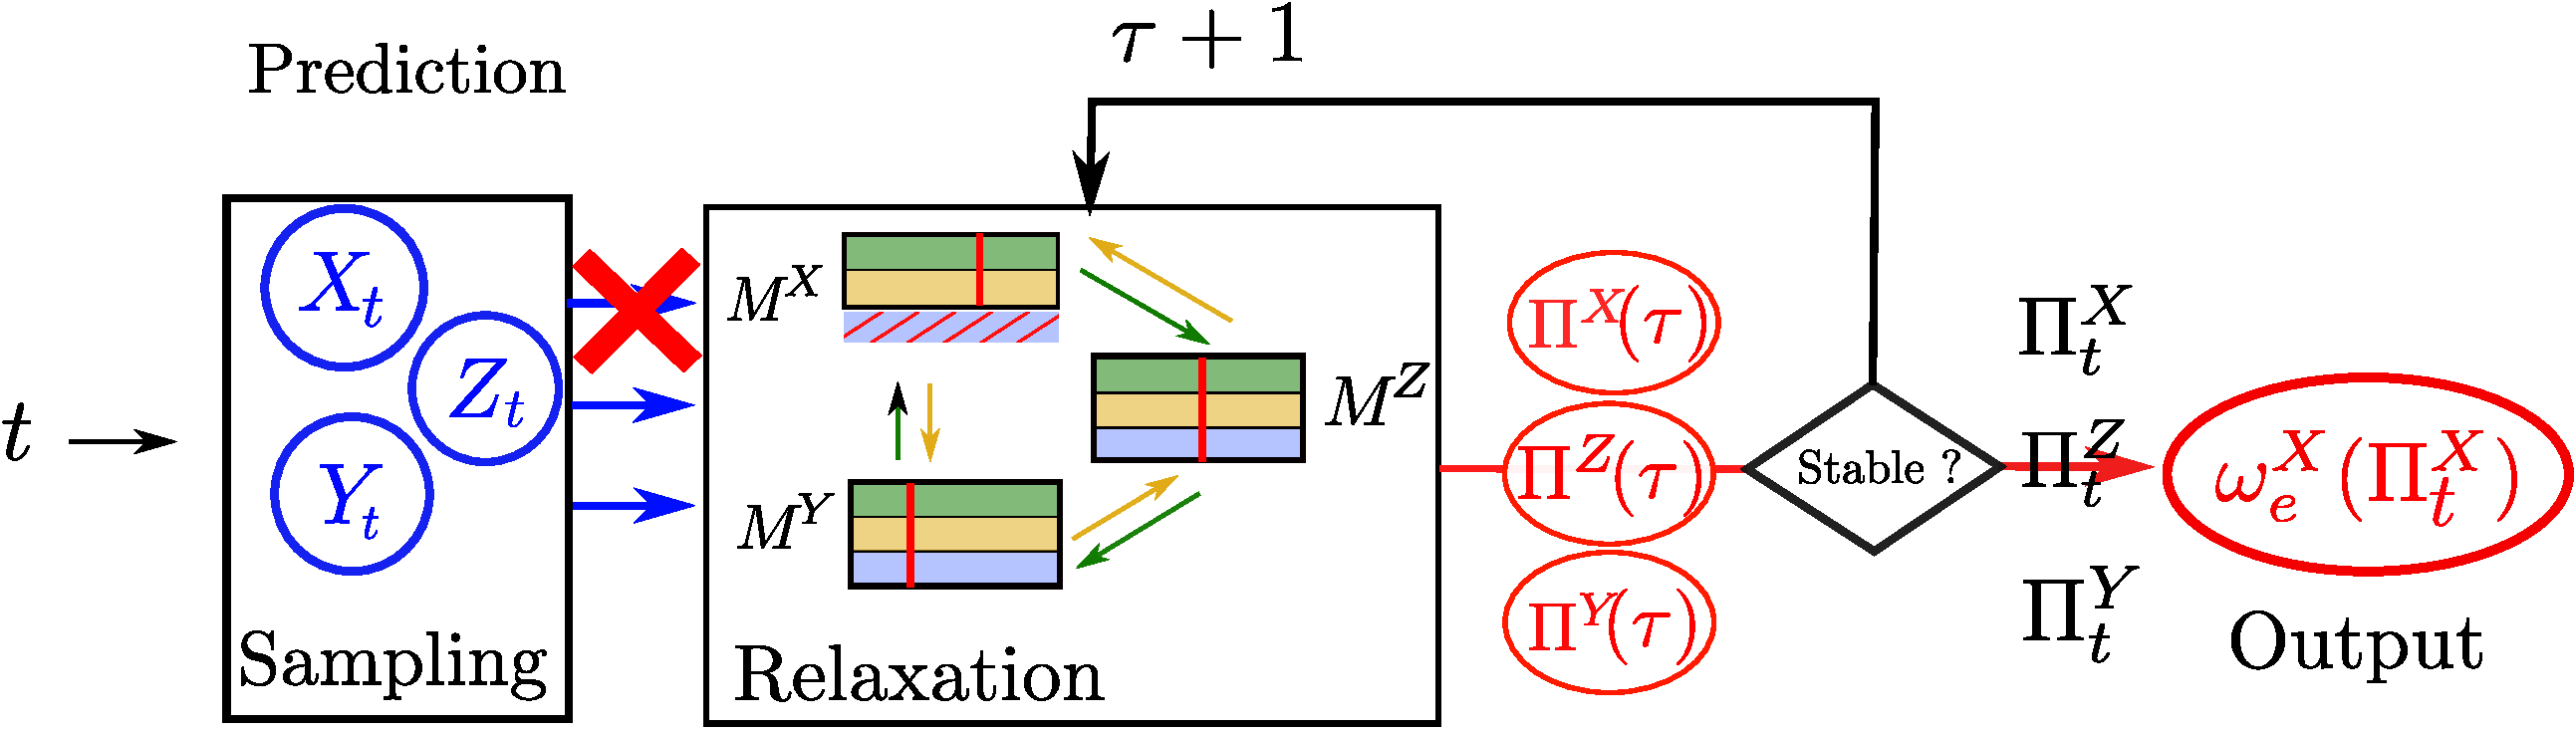
\includegraphics[width=\textwidth]{prediction_setup}
\caption{Description de l'algorithme de prédiction. Il s'agit du même algorithme que pour les tests, sans apprentissage, mais une modalité n'est pas présentée à l'architecture.}
\label{fig:schema}
\end{figure}


\subsection{Résultats}

La figure \ref{fig:pred} représente la valeur de la prédicton $\w\ext\m{1}(\bmu\m{1})$ en fonction de la valeur théorique de cette entrée. 
\begin{figure}
\centering
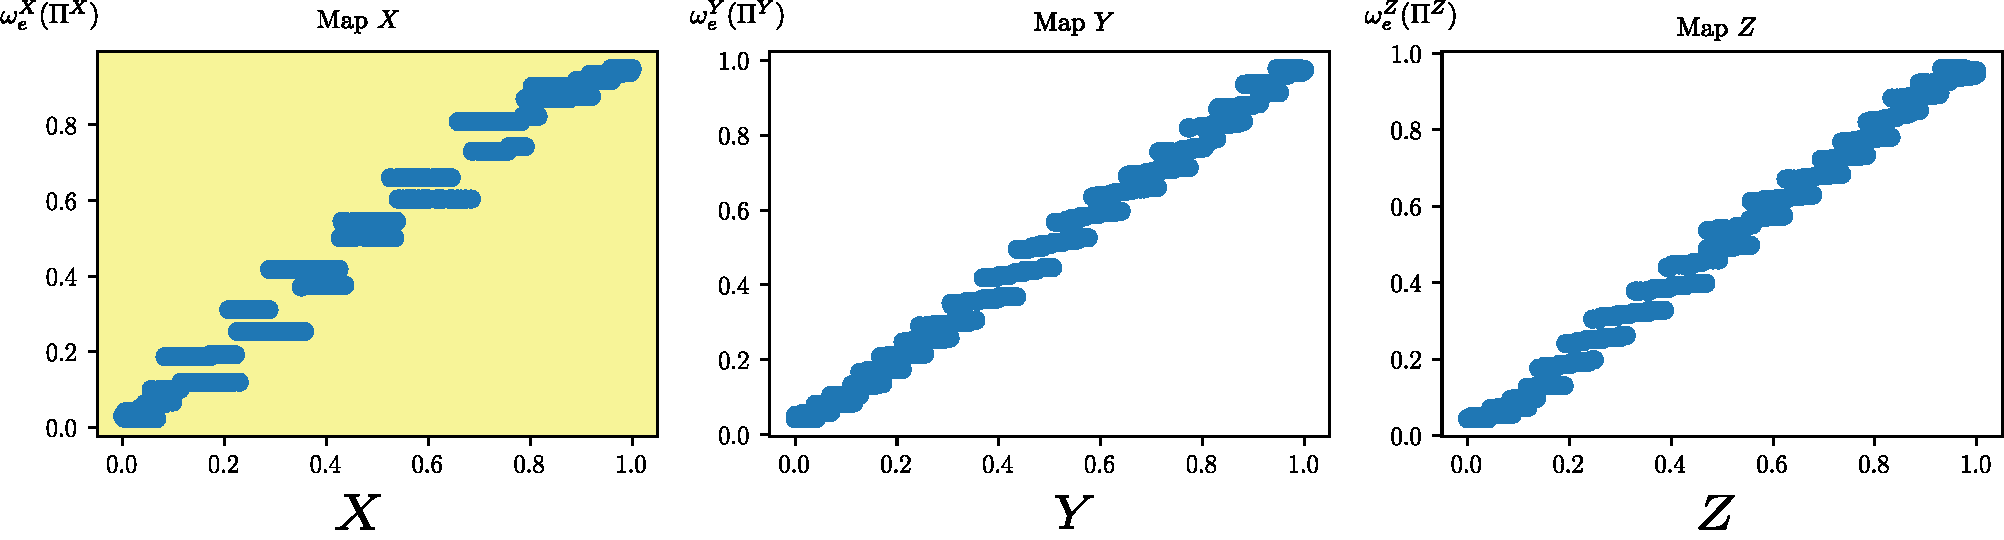
\includegraphics[width=\textwidth]{prediction_x2}
\caption{Prediction de x}
\label{fig:pred}
\end{figure}


\subsection{Discussion}
Les résultats sur des entrées géométriques montrent une bonne capacité de prédiction d'entrée.
La précision est limitée, mais on peut voir cette capacité de prédiction plus comme une preuve de mémoire associative que d'application pratique.
Ce qu'on cherche par la mémoire associative, c'est d'abord d'évoquer une modalité à partir d'autres. Ici, grâce à la connexion entre carte, on génère une zone de valeur limitée pour la modalité $X$: une région est activée, qui est reliée aux valeurs de $X$.
On va plutot parler d'évocation plutot que de prédiction. 

\section{Application à la commande de drône en vol}

Nous appliquobns maintenant cette méthode de prédiction pour la commande d'un drône en vol. Nous disposons d'un drône quadricoptère, commandé à distance. Nous utiliserons la prédiction à l'aide de CxSOM pour que le drône reste centré dans un couloir lors d'un vol en ligne droite. 

Après demi tour, stabilisation nécessaire : on est dans une situation ou on a quand même besoin d'une correction de trajectoire.
But de l'expérience: preuve du concept en situation réelle; évaluation de la robustesse au bruit et aux données réelles; évaluation de la capacité de CxSOM à réagir rapidement malgré les calculs.

\subsection{Méthode expérimentale}

\begin{figure}
\begin{minipage}{0.5\textwidth}
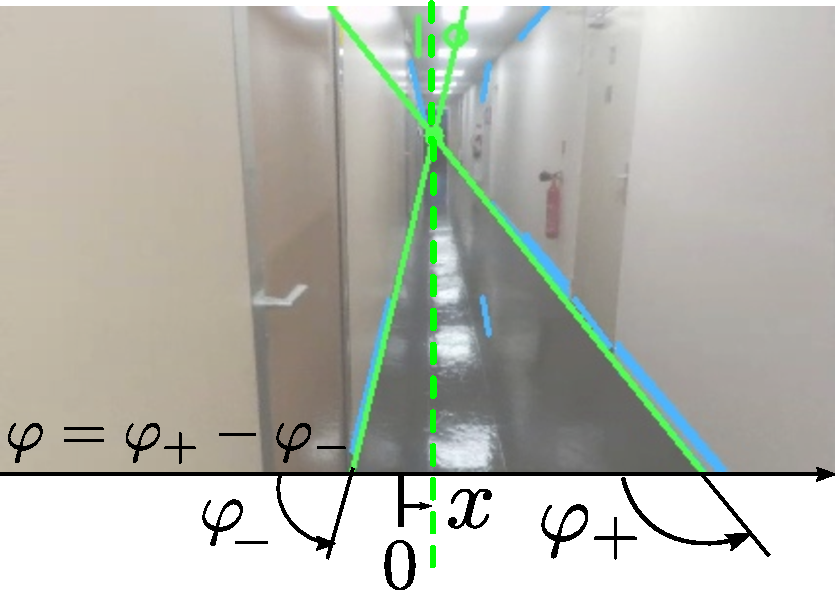
\includegraphics[width=\textwidth]{visudrone}
\end{minipage}
\begin{minipage}{0.5\textwidth}
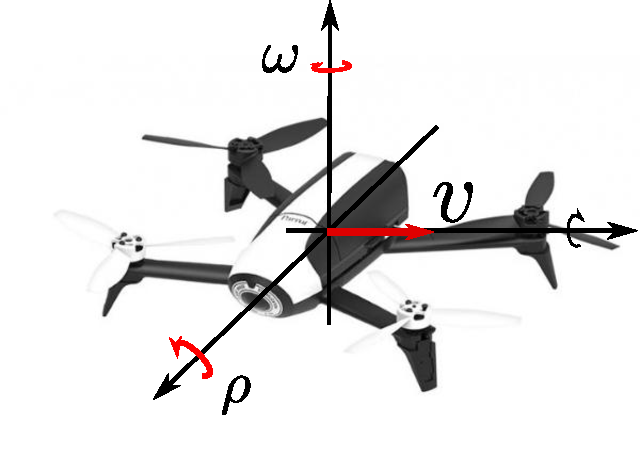
\includegraphics[width=\textwidth]{dronesteup}
\end{minipage}
\caption{Disposition des capteurs utilisés pour l'experience}
\end{figure}


\subsection{Résultats}

\begin{figure}
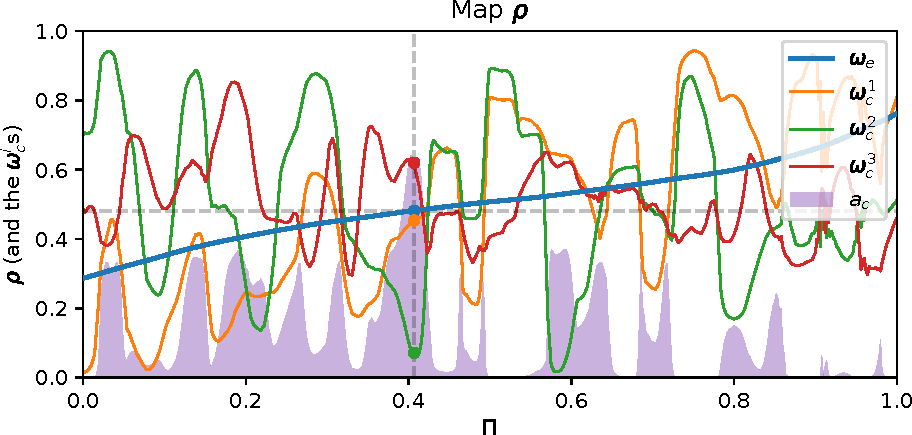
\includegraphics[width=\textwidth]{dronemap}
\caption{Disposition des poids de la carte $\rho$ après apprentissage et exemple de calcul d'activité}
\end{figure}

Vidéos de test disponibles sur un répertoire ?

\subsection{Discussion}
Ici on ne cherchait pas à comparer avec des valeurs théorique, mais on observe que le drone ne tape pas les murs
Illustration de la capacité de prédiction et mémoire associative
Resistance au bruit

Calcul des dépendance entre les entrées et la commande:
PCA sur les entrées, calcul de MI après apprentissage
\section{Conclusion}





